\documentclass[12pt,aspectratio=169]{beamer}

\usetheme[
    sectionpage=progressbar,
    subsectionpage=progressbar,
    progressbar=frametitle
]{metropolis}

\definecolor{mDarkBrown}{HTML}{FF5722}
\definecolor{mDarkTeal}{HTML}{263238}
\definecolor{mLightBrown}{HTML}{FF5722}

\usepackage{booktabs}
\usepackage{graphicx}
\usepackage{hyphenat}
\usepackage{multirow}
\usepackage[normalem]{ulem}

\usepackage{pifont}
\newcommand{\cmark}{\ding{51}}
\newcommand{\xmark}{\ding{55}}

\usepackage{polyglossia}
\setdefaultlanguage[variant=british]{english}
\usepackage[english=british]{csquotes}

\defaultfontfeatures{Ligatures=TeX}
\setmainfont{Lucida Sans OT}
\setsansfont[Scale=MatchLowercase]{Lucida Sans OT}
\setmonofont[Scale=MatchLowercase]{Lucida Console DK}

\author{Gianluca Campanella}
\date{}



\title{Introduction to complex networks}

\newcommand{\set}[1]{\ensuremath{\mathcal{#1}}}

\renewcommand{\vec}[1]{\ensuremath{\mathbf{#1}}}
\newcommand{\mat}[1]{\ensuremath{\vec{#1}}}
\newcommand{\tr}{\ensuremath{\intercal}}

\newcommand{\R}{\ensuremath{\mathbb{R}}}
\newcommand{\N}{\ensuremath{\mathcal{N}}}

\begin{document}

\maketitle

\begin{frame}{Contents}
    \tableofcontents[hideallsubsections]
\end{frame}

\section{Definitions}

\begin{frame}{Graph theory}
    \begin{description}
        \item[1736] Euler writes the first paper
        \item[1959] Erdős and Rényi introduce probabilistic methods
    \end{description}
    \vfill
    \begin{center}
        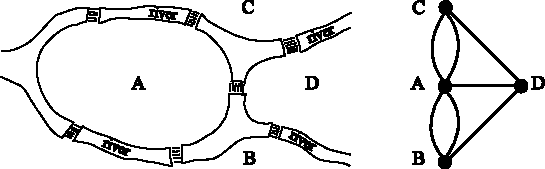
\includegraphics[height=10em]{figures/seven_bridges} \\
        {\scriptsize%
         From Junker and Schreiber (2008)}
    \end{center}
\end{frame}

\begin{frame}{Network theory}
    \begin{description}
        \item[1970s] Sociologists (`social network analysis')
        \item[2000s] Physicists and Computer Scientists
    \end{description}
    \vfill
    \begin{center}
        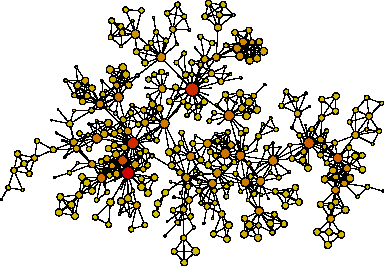
\includegraphics[height=10em]{figures/network}
    \end{center}
\end{frame}

\begin{frame}{Graphs and their representation}
    A graph $\set{G} = \left( \set{V}, \set{E} \right)$ consists of:
    \begin{enumerate}
        \item a set of \textbf{vertices}
              $\set{V} = \left\{ v_{1}, \ldots, v_{n} \right\}$
        \item a binary relation $\set{E} \subseteq \set{V}^{2}$ that represents
              \textbf{edges}
    \end{enumerate}
    \vfill\pause
    \begin{block}{Alternative representation of $\set{E}$}
        In terms of the \textbf{adjacency matrix}
        $\mat{A} \in \{ 0, 1 \}^{n \times n}$, with elements
        \[
            a_{ij} =
            \begin{cases}
                1 & \text{if} \left( v_{i}, v_{j} \right) \in \set{E} \\
                0 & \text{otherwise}
            \end{cases}
        \]
    \end{block}
\end{frame}

\begin{frame}{Example}
    \begin{columns}
        \begin{column}{0.5\textwidth}
            \begin{center}
                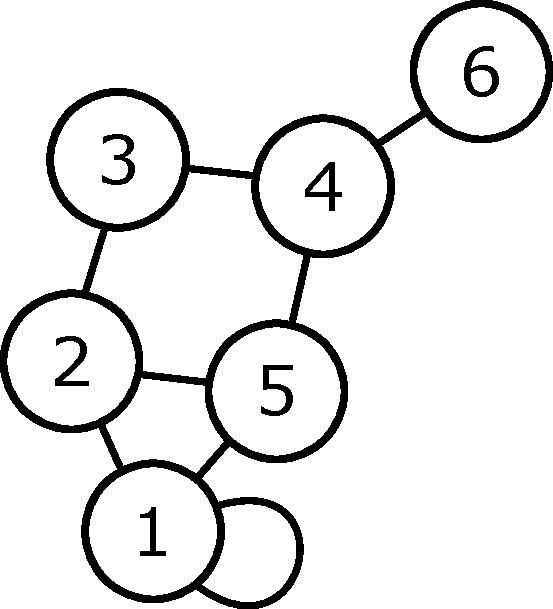
\includegraphics[height=0.85\textheight]{figures/graph}
            \end{center}
        \end{column}
        \begin{column}{0.5\textwidth}
            \vspace{1em}
            \begin{align*}
                \set{V} &= \left\{ v_{1}, \ldots, v_{6} \right\} \\
                \set{E} &= \left\{ (v_{1}, v_{1}), (v_{1}, v_{2}), \ldots \right\} \\[1em]
                \mat{A} &=
                \begin{pmatrix}
                    1 & 1 & 0 & 0 & 1 & 0\\
                    1 & 0 & 1 & 0 & 1 & 0\\
                    0 & 1 & 0 & 1 & 0 & 0\\
                    0 & 0 & 1 & 0 & 1 & 1\\
                    1 & 1 & 0 & 1 & 0 & 0\\
                    0 & 0 & 0 & 1 & 0 & 0\\
                \end{pmatrix}
            \end{align*}
        \end{column}
    \end{columns}
\end{frame}

\begin{frame}{Weights}
    \begin{itemize}
        \item Assigned to elements of \set{E}
        \item Represent the \textbf{strength} of the relationship
    \end{itemize}
    \vfill
    \begin{block}{Examples}
        \begin{itemize}
            \item Signed edges:
                  $\mat{A} \in \{ -1, 0, 1 \}^{n \times n}$
            \item Weights on the unit interval:
                  $\mat{A} \in [ 0, 1 ]^{n \times n}$
            \item Weights on the positive real line:
                  $\mat{A} \in [ 0, \infty )^{n \times n}$
        \end{itemize}
    \end{block}
\end{frame}

\begin{frame}{Properties of $\set{E}$}
    \begin{block}{Irreflexivity}
        \centering
        $\forall\, v_{i} \in \set{V}.\, (v_{i}, v_{i}) \not \in \set{E}$
        \begin{itemize}
            \item[$\rightarrow$] No `self\hyp{}loops' allowed
        \end{itemize}
    \end{block}
    \vfill
    \begin{block}{Symmetry}
        \centering
        $\forall\, v_{i}, v_{j} \in \set{V}.\, (v_{i}, v_{j}) \in \set{E} \Rightarrow (v_{j}, v_{i}) \in \set{E}$
        \begin{itemize}
            \item[$\rightarrow$] Direction of the relationship does not matter
                                 ($\set{G}$ is \textbf{undirected})
            \item[$\rightarrow$] $\mat{A} = \mat{A}^{\tr}$ is also symmetric
        \end{itemize}
    \end{block}
\end{frame}

\begin{frame}{Properties of vertices}
    \begin{block}{Neighbourhood}
        \centering
        $\N(v_{i}) = \left\{ v_{j} : (v_{i}, v_{j}) \in \set{E} \right\} \subseteq \set{V}$
        \begin{itemize}
            \item[$\rightarrow$] \textbf{Set} of vertices to which $v_{i}$ is
                                 connected by edges
        \end{itemize}
    \end{block}
    \vfill
    \begin{block}{Degree}
        \centering
        $k_{i} = k(v_{i}) = \left| \, \N(v_{i}) \, \right|$
        \begin{itemize}
            \item[$\rightarrow$] \textbf{Number} of vertices to which $v_{i}$ is
                                 connected by edges
        \end{itemize}
    \end{block}
\end{frame}

\begin{frame}{In- and out-degree}
    \begin{columns}
        \begin{column}{0.5\textwidth}
            \begin{align*}
                k^{\text{in}}_{i} &= \left| \left\{ \left( v_{j}, v_{i} \right)\;\middle|\;\left( v_{j}, v_{i} \right) \in \set{E} \right\} \right| \\[1em]
                k^{\text{out}}_{i} &= \left| \left\{ \left( v_{i}, v_{j} \right)\;\middle|\;\left( v_{i}, v_{j} \right) \in \set{E} \right\} \right|
            \end{align*}
        \end{column}
        \begin{column}{0.5\textwidth}
            \begin{center}
                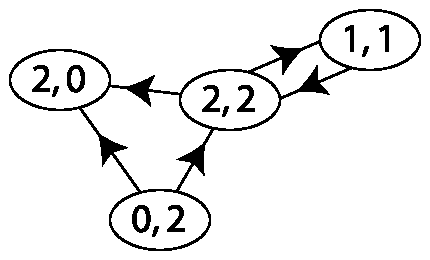
\includegraphics[width=\textwidth]{figures/degree}
            \end{center}
        \end{column}
    \end{columns}
\end{frame}

\begin{frame}{Paths}
    \only<1>{%
        A \textbf{path} on $\set{G} = ( \set{V}, \set{E} )$ is a graph
        $\set{P} = ( \set{V}_{\set{P}}, \set{E}_{\set{P}} )$ with:
        \begin{enumerate}
            \item $\set{V}_{\set{P}} = \{ v_{(0)}, \ldots, v_{(l)} \} \subseteq \set{V}$
            \item $\set{E}_{\set{P}} = \{ (v_{(0)}, v_{(1)}), \ldots, (v_{(l-1)}, v_{(l)}) \} \subseteq \set{E}$
        \end{enumerate}
        \begin{description}
            \item[Ends] Vertices $v_{(0)}$ and $v_{(l)}$
            \item[Length] Number of edges
                          $\left| \, \set{E}_{\set{P}} \, \right| = l$
        \end{description}}
    \only<2>{%
        \begin{center}
            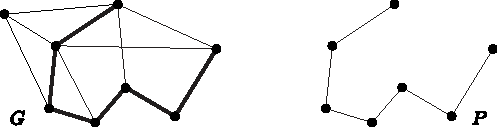
\includegraphics[width=\textwidth]{figures/path} \\[1em]
            {\scriptsize%
             From Diestel (2010)}
        \end{center}}
\end{frame}

\begin{frame}{Shortest paths}
    \begin{center}
        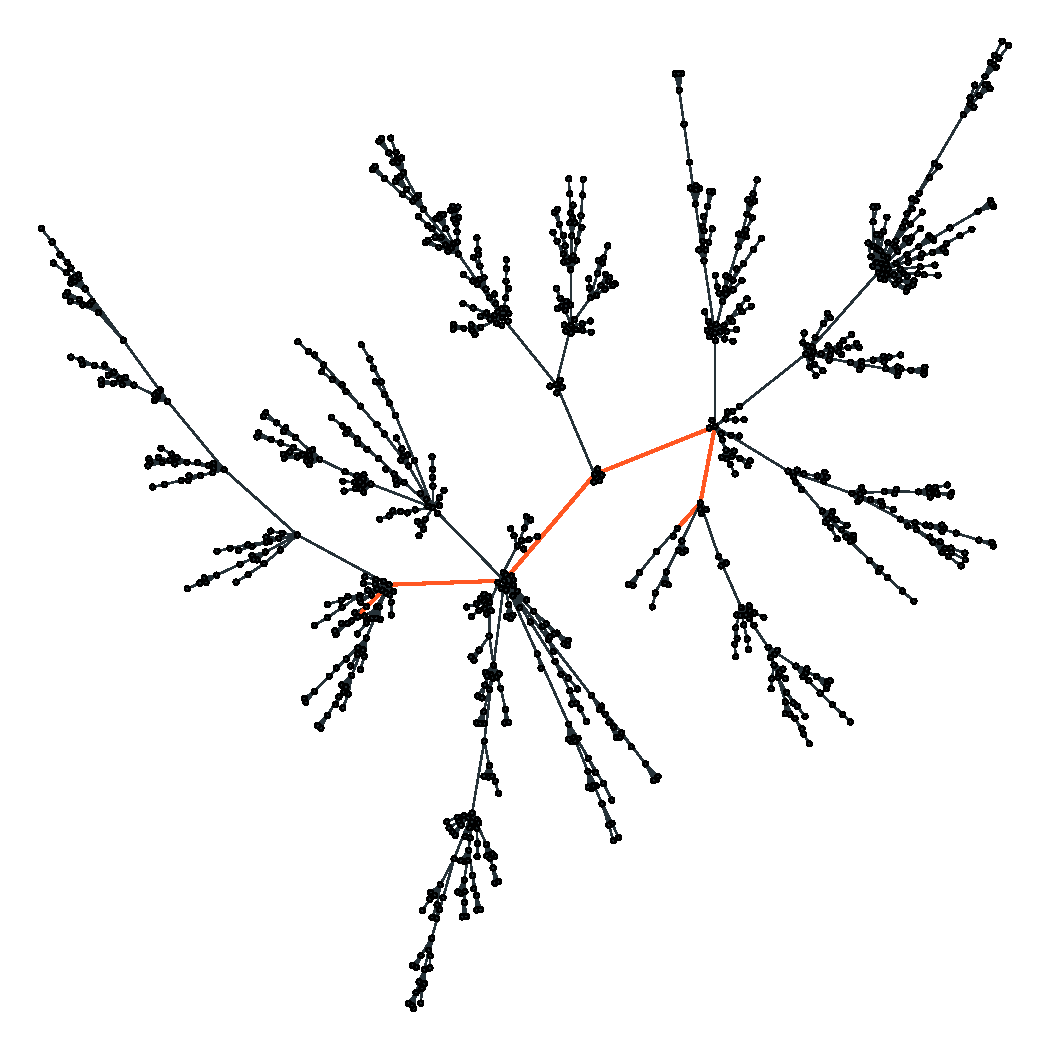
\includegraphics[height=0.85\textheight]{figures/shortest_path}
    \end{center}
\end{frame}

\section{Local properties}

\begin{frame}{Centrality}
    \begin{center}
        \Large%
        Which are the most important \\
        (or `central') vertices?
    \end{center}
    \vfill
    \only<1>{%
        \begin{block}{Degree centrality}
            How many connections does a vertex have to other vertices?
        \end{block}}
    \only<2>{%
        \begin{block}{Closeness centrality}
            How `far' (in terms of shortest paths) is a vertex with respect to
            all other vertices?
        \end{block}}
    \only<3>{%
        \begin{block}{Betweenness centrality}
            How many times does a vertex act as a `bridge' along the shortest
            paths between all pairs of vertices?
        \end{block}}
    \only<4>{%
        \begin{block}{Eigenvector centrality (PageRank)}
            How many times do we stumble upon a vertex while randomly walking on
            the graph?
        \end{block}}
\end{frame}

\begin{frame}{Local clustering coefficient}
    \[
        C_{i} = C(v_{i}) = \frac{| \, \{ (v_{j}, v_{k}) : \{ (v_{i}, v_{j}), (v_{i}, v_{k}), (v_{j}, v_{k}) \} \subseteq \set{E} \} \, |}{k_{i} \, (k_{i} - 1) / 2} \in [0, 1]
    \]
    \vfill
    \begin{itemize}
        \item Probability that a pair of neighbours of $v_{i}$ are connected
        \item Empirically: $k_{i} \nearrow$, $C_{i} \searrow$
        \item[$\rightarrow$] Can be used to identify `structural holes'
    \end{itemize}
\end{frame}

\section{Large-scale structure}

\begin{frame}{`Small-world' effect}
    \vfill
    \begin{quotation}
        `\ldots Milgram's letter\hyp{}passing experiment in the 1960s, in which
        people were asked to get a letter from an initial holder to a distant
        target person by passing it from acquaintance to acquaintance through
        the social network.
        The letters that made it to the target did so in a remarkably small
        number of steps, around six on average.'

        \begin{flushright}
            \scriptsize%
            From Newman (2010)
        \end{flushright}
    \end{quotation}
    \vfill
\end{frame}

\begin{frame}{Degree distribution}
    \[
        \Pr\!\left[ K = k \,\right]
        = \Pr\!\left[ \text{`a randomly selected vertex $v_{i} \in \set{V}$ has degree $k \geq 0$'} \right]
    \]
    \begin{center}
        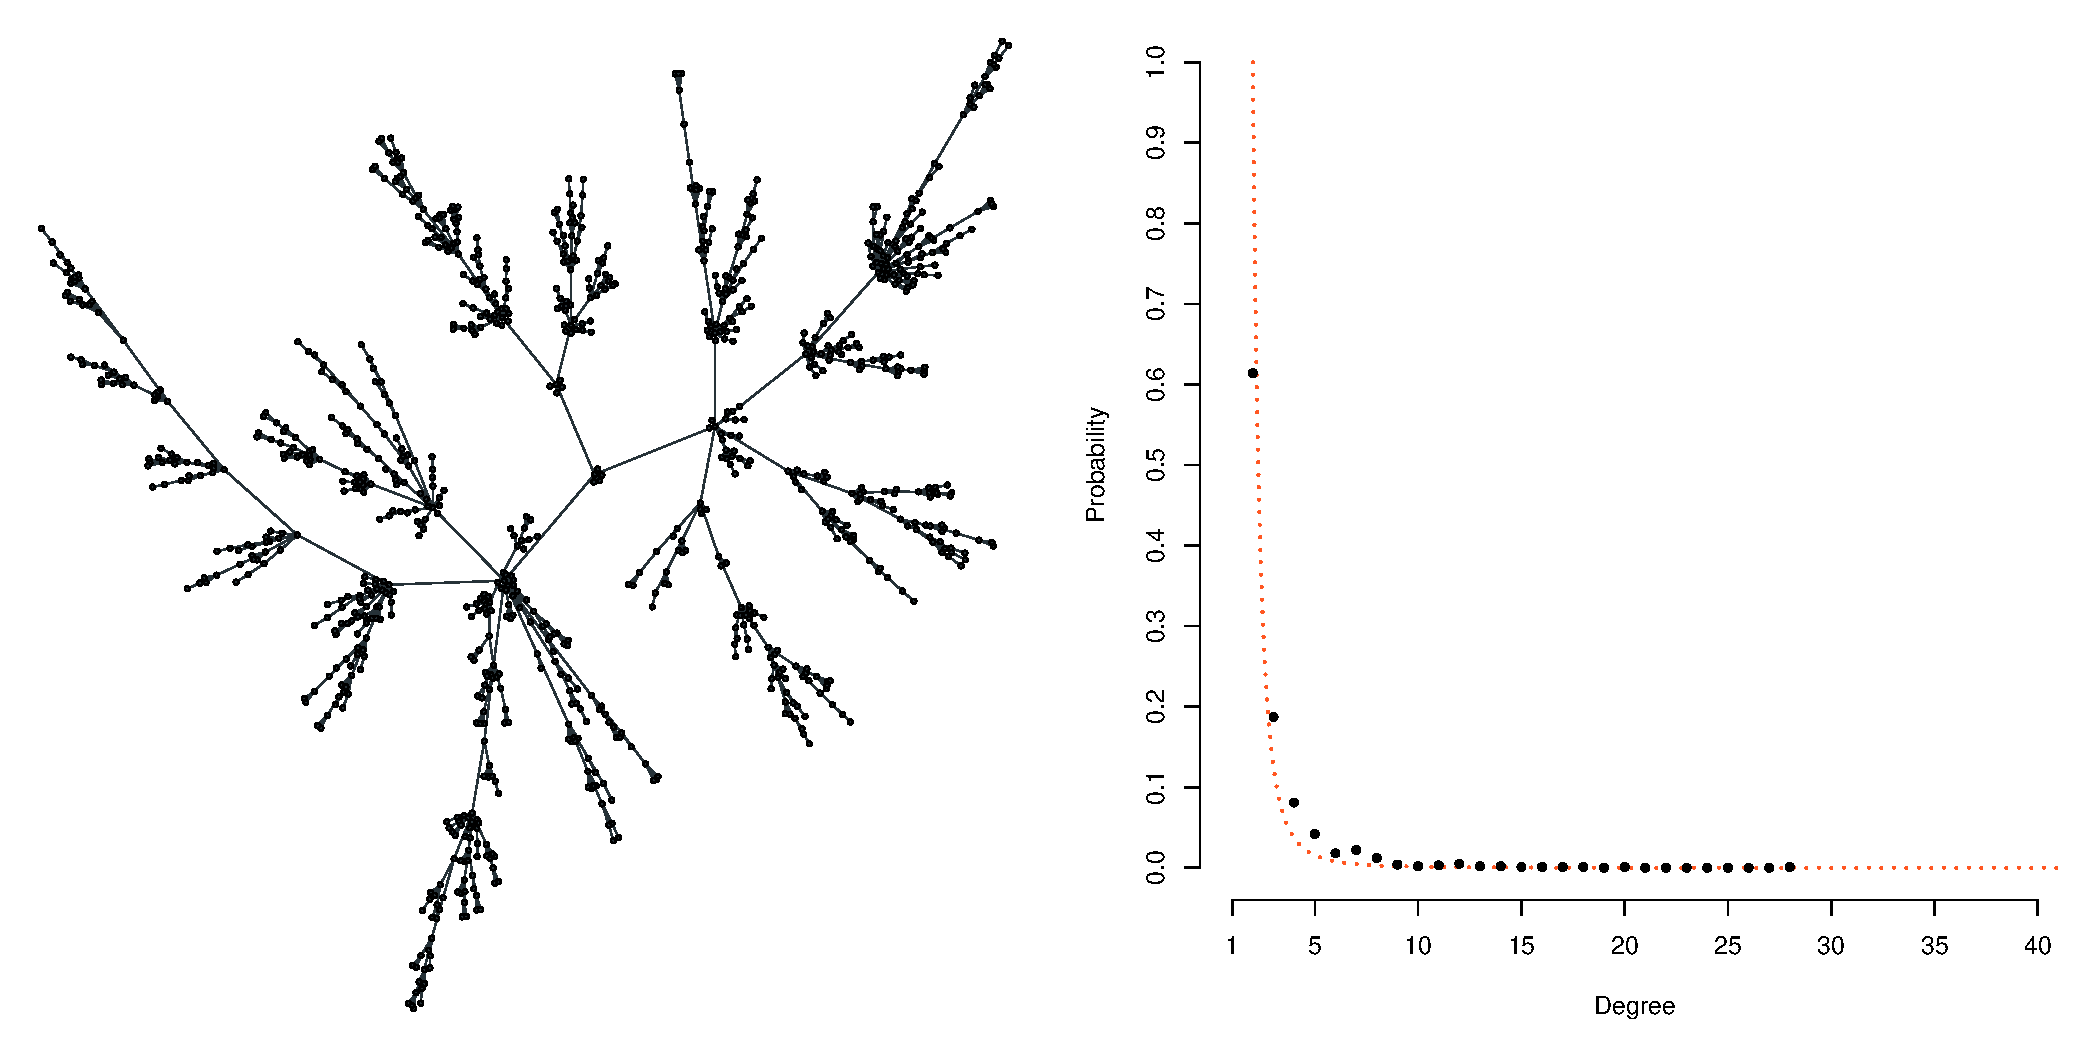
\includegraphics[height=0.65\textheight]{figures/degree_dist}
    \end{center}
\end{frame}

\begin{frame}{Power laws}
    \begin{align*}
        \ln y &= - \alpha \ln x + c \\
        y &= C\,x^{\,-\alpha}, \quad C = e^{\,c}
    \end{align*}
    \vfill
    \begin{itemize}
        \item Sizes of city populations and wars
        \item Frequency of use of words in human languages
        \item Occurrence of personal names in most cultures
        \item Number of papers scientists write
        \item Number of hits on Web pages
        \item Sales of almost every branded commodity
        \item Number of species in biological taxa
    \end{itemize}
\end{frame}

\begin{frame}{Scale-free networks}
    \only<1>{%
        \begin{itemize}
            \setlength{\itemsep}{\bigskipamount}
            \item $\Pr\!\left[ K = k \,\right] \propto k^{\,-\alpha}$
                  (at least asymptotically), usually $2 \le \alpha \le 3$
            \item \textbf{Self\hyp{}similar} (scale invariance)
            \item Presence of \textbf{hubs} (Milgram's `sociometric superstars')
                  \begin{itemize}
                      \item[$\rightarrow$] Fault tolerance
                      \item[$\rightarrow$] `Small\hyp{}world' effect
                  \end{itemize}
        \end{itemize}}
    \only<2>{%
        \begin{block}{Examples}
            \begin{itemize}
                \setlength{\itemsep}{\medskipamount}
                \item Social and collaboration networks
                \item Many kinds of communication networks (e.g.\ the Internet)
                \item \textbf{Many biological networks}
            \end{itemize}
        \end{block}}
\end{frame}

\section{Models of network formation}

\begin{frame}{What is complexity?}
    \only<1>{%
        \begin{block}{Complex}
            Many interacting parts, not necessarily `difficult'
        \end{block}
        \vfill
        \begin{block}{Complicated}
            Difficult, not necessarily `complex'
        \end{block}}
    \only<2>{%
        \begin{center}
            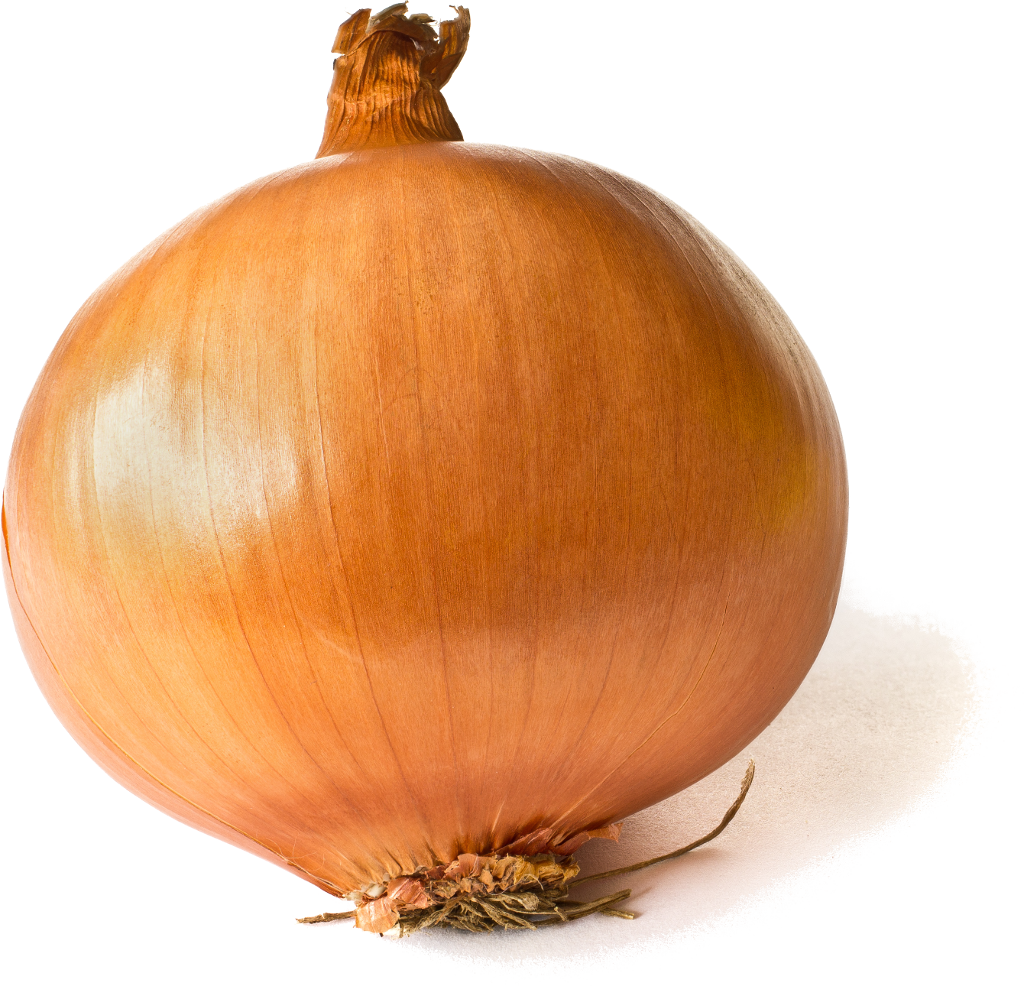
\includegraphics[height=0.8\textheight]{figures/onion} \\
            {\scriptsize%
             Via \textit{Wikimedia Commons}}
        \end{center}}
\end{frame}

\begin{frame}{Self-organisation}
    \only<1>{%
        \begin{center}
            \Large%
            Spontaneous emergence of global structure \\
            out of local interactions
        \end{center}
        \begin{itemize}
            \setlength{\itemsep}{\medskipamount}
            \item Robust to damage and perturbations
                  \begin{itemize}
                      \item Not controlled by (internal or external) agents
                      \item Collective, distributed process
                  \end{itemize}
            \item Outcome is not arbitrary, but `prefers' certain situations \\
                  $\rightarrow$ Natural selection
        \end{itemize}}
    \only<2>{%
        \begin{block}{Examples}
            \setlength{\itemsep}{\medskipamount}
            \begin{itemize}
                \item Protein folding
                \item Pattern formation and morphogenesis
                \item Social structures and herd behaviour
            \end{itemize}
        \end{block}}
    \only<3>{%
        \begin{center}
            \Large%
            Topology is crucial to understanding \\
            stochastic processes on networks
        \end{center}}
\end{frame}

\begin{frame}{Models of network formation}
    \begin{center}
        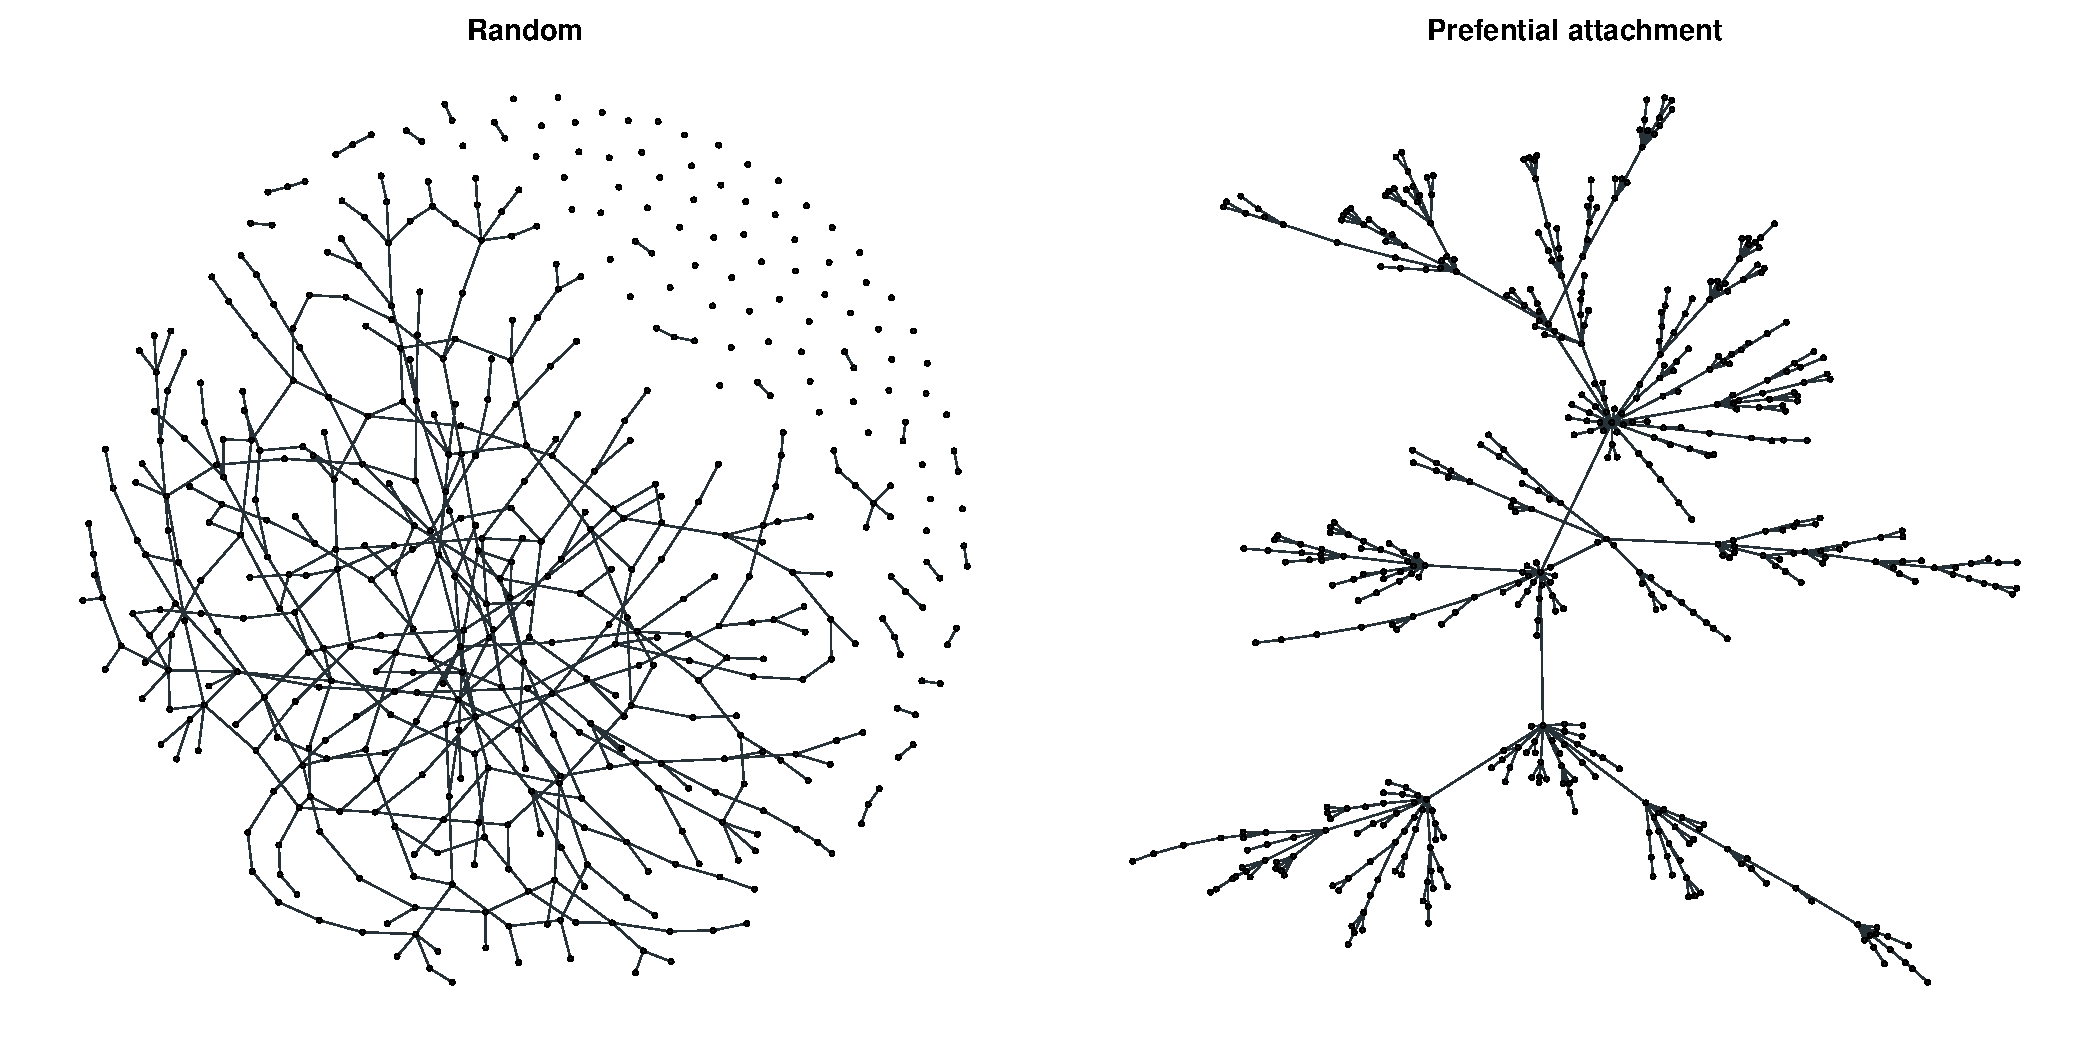
\includegraphics[width=\textwidth]{figures/models}
    \end{center}
\end{frame}

\begin{frame}{Erdős--Rényi model}
    \begin{block}{Algorithm}
        Construct a graph with $n$ vertices and include each edge with
        probability $p$ (independently from every other edge)
    \end{block}
    \vfill\pause
    \begin{block}{Degree distribution}
        \[
            \Pr\left[ K = k \,\right] = \binom{n-1}{k} \, p^{\,k} \left( 1-p \right)^{\,n-1-k}
        \]
    \end{block}
\end{frame}

\begin{frame}{Barabási--Albert model}
    \begin{block}{Algorithm}
        \begin{itemize}
            \item Start with an initial connected graph with $n$ vertices
            \item Add a new vertex and connect it to $n^{\star} \leq n$ existing
                  vertices with probability proportional to their degree \\
                  $\rightarrow$ \textbf{Preferential attachment}
        \end{itemize}
    \end{block}
    \vfill\pause
    \begin{block}{Degree distribution}
        \[
            \Pr\left[ K = k \,\right] \propto k^{\,-3}
        \]
    \end{block}
\end{frame}

\begin{frame}{What about `--omics'?}
    \begin{itemize}
        \setlength{\itemsep}{\bigskipamount}
        \item Very few longitudinal datasets \\
              $\rightarrow$ Difficult to understand evolution
        \item Few cross\hyp{}platform studies \\
              $\rightarrow$ Can understand interactions between complexity
                            levels
        \item Many single\hyp{}platform studies \\
              $\rightarrow$ Can characterise ``co\hyp{}'' networks
    \end{itemize}
\end{frame}

\end{document}

